\section{Design}
\label{sec:design}

% this section is used to discuss the design considerations of the system
% starting from a motivating example, and then extract the key requireements, then about system design

In this section, we will talk about our design considerations in solving the ``addressing'' problem in the smart environment. We start by describing the example application, where in an ideal case, how the user should interact with physical devices. From that, we draw some design requirements. To explore the design space, we propose several possible solutions. Some of them are difficult to achieve within a shrot time. In next section, we will build a proof-of-concept system, where we have simplified several tasks.

\subsection{Example Application}
\label{sec:example-application}

Our work is primarily motivated by the observation that in CS294-84 course at Berkeley, the instructor has to go to the switch to turn off the light during presentation. The separation of device and their controller makes it possible for people control things that are not reachable (such as the lights on the ceiling). However, such indirection introduces additional overhead since people still need to locate the controller and then interact. Remote control might mitigate such a problem, but one controller for one device is not a scalable solution. And squeezing controllers onto the smartphone display is also not the right approach. We will demonstrate this by giving the following Smart Home example.

% {\bf Smart Home}:
% Sean, maybe you can elaborate on this application more to motivate.
Imagine in a smart-home environment that most devices are remotely controllable. When the users are watching TV shows, they want to turn off the lights and turn up the volume so they can enjoy this memorable time. Such ordinary-life tasks are happening everyday, and any simplification will result in significant time savings. One ideal approach is that the user expresses his interest of turning off the lights by simply staring at the light, plus a specific gesture. Then he turns his head back to the TV, and again simply ``asks'' the TV to turn up the volume. When transitioning, the disconnection with the light and the connection with TV happens seamlessly, with the correct feedback for the user. And all the magic are resolved by an always-available device; this might be the glasses, rings or watches. 

Occasionally, the user needs to perform some advanced configurations to the TV, such as adjusting the white balance, or the brightness. Since the need of these complicated tasks are not frequent, and it will be less efficient to embed these features into the always-available device (which is designed to be small and easy-to-access, rather than too flexible). The smart-home falls back to a more generic approach which relies on touch screen or other rich input device. In this example case, since the user's attention is still on TV, his smartphone may pop up the control menu for advanced usage automatically. Such menu could also just pop up on walls or other large interactive displays \cite{unPad:eWallpaper, MSVision}. Even in this case, the attention system knows users' intention and saves time for user to address the device to interact.

\subsection{System Requirements}
\label{sec:system-requirements}

From what we have described in the previous section, the example application is enabled by a few necessary requirements. We will discuss some important ones in this section.

% leads to the adoption of glass
The first and foremost is the ability to sense and control in an always-available fashion. Since the goal is to simplify everyday task in a smart-home or smart-office scenario, any cubersome solution is not desired. The control of the device would also have to be simple, not to confuse the user of using it. 

Secondly, since screens might not always be available when users are interacting directly with physical device. Adequate feedback should assist user understanding what is going on. Even if screens are everywhere to assist in the future, the requirements of having proper feedback still hold.

As discussed before, we envision the simple always-available device would not be capable to cover all tasks. For those which are really complicated and less likely being executed, we will have to enable the system to fall back.

Besides the previous three, for any human-centric system, additional requirements like responsiveness would also be required, though not explicit discussed through this paper.

\subsection{System Design}
\label{sec:system-design}

In this section, we will present several design consideration that fulfills the requirements. From \cite{Merrill:2007:ALP:1758156.1758158}, they tried the solution of putting IR into earphones, rings to enable looking, pointing and reaching metaphor. When we were thinking about how to capture user's attention, we are actually leaning towards the glasses solution. Part of the motivation is from Google Glass. Generally, glasses are more natural in align with human's light of sight. Therefore, sensors on glasses can reflect the users' attention in a more precise way. Then given the glass form factor, what might be the right sensor or component to use to obtain users' attention remains a major question for us.

The first possible approach is a pure Google Glass solution. Since the glasses come with a camera, sophiscated computer vision algorithms might be able to detect what is in front of the user's sight. Following this thoughts, the camera would also be able to tell users' gestures. In fact, there are more features which would make this interaction cooler -- the voice recognition is another important source of user input, the projection onto user's eyeballs can provide timely feedback to users' action, the networking capability provide seamless connection with other peripheral devices such as displays. And initially, we were also thinking about building a prototype that resembles Google Glass, but the complexity behind of achieving acceptable image processing is huge. Not to mention we don't have the Google Glass yet. This approach is more an exploration of design space. 

Since our target is to validate the thoughts of interacting directly with physical objects through users' attention. We might break the initial proposal to several achievable tasks and build the proof-of-concept. Our second approach still adopts the glass form factor, but we've turned to other sensors to detect users' line of sight. 

Specifically, we choose to use IR. When surrounded by tubes, the IR is pretty directional. And from our test, it can differentiate objects in {\color{red} 20 (do some experiments here)} centimeters. User input can be captured by a slider on glass frame, where it's easy to access (though not hand-free). The networking capability is enabled by having an XBee module on the main board. We propose the interaction architecture in Fig.\,\ref{fig:sysarch}.

\begin{figure}
  \centering
  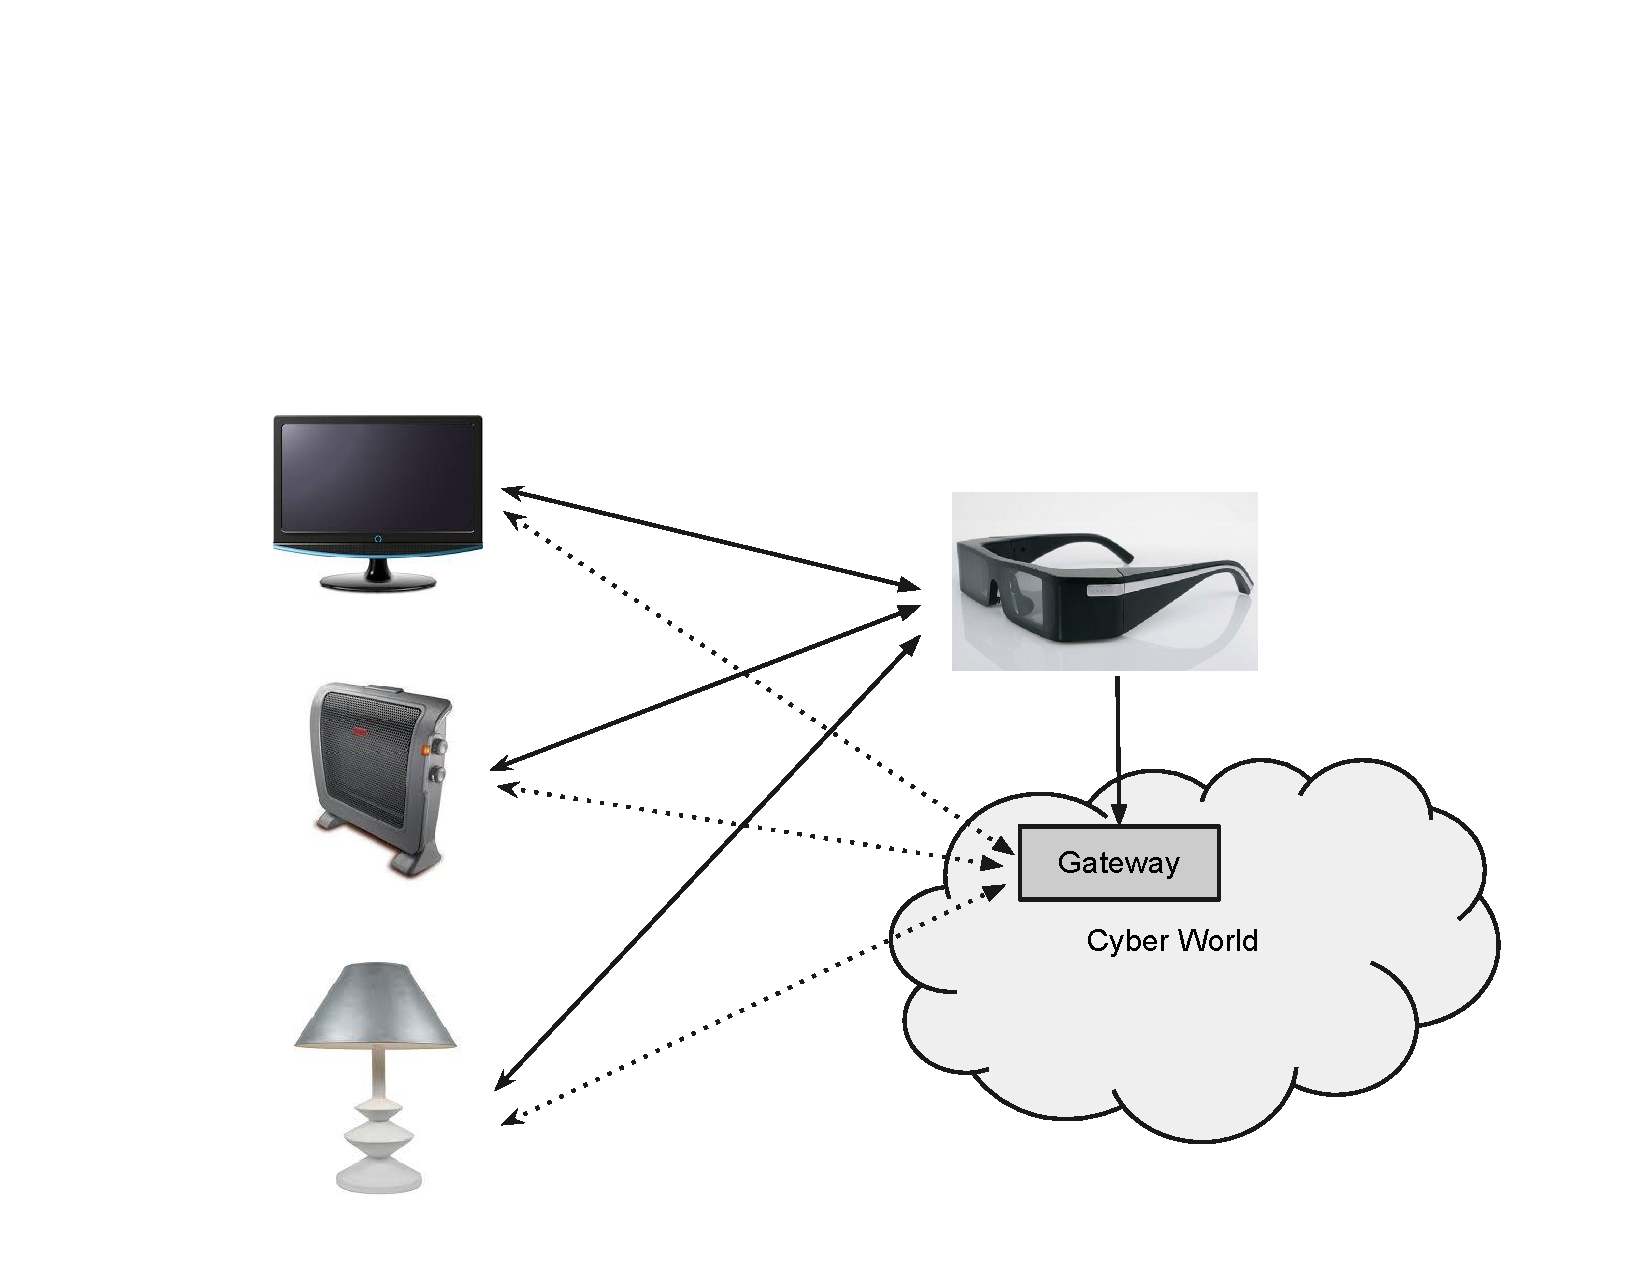
\includegraphics[width=\linewidth]{../figs/sysarch.pdf}
  \caption{System Architecture}
  \label{fig:sysarch}
\end{figure}

The dotted lines show some existing (even gradually commercialized) approaches that seek to provide access to physical objects through gateways from the broader Internet. In our project, we focus on the solid lines where the users can interact with them directly. Also as has been pointed out in the requirements, the fall-back scheme for complicated tasks are enabled by the communication between the glasses and the gateway. Though simple enough, we find it essentially useful to have this architectural figure in mind when considering users' interaction.


% Lessons learned from \cite{Bellotti:2002:MSS:503376.503450} have also guided us in thinking the Five A's when designing novel interaction system. 


%%% Local Variables: 
%%% mode: latex
%%% TeX-master: "main"
%%% End: 

